\section{Kurzbeschreibung}
Diese Anleitung dient dem Aufbau sowie dem Einsatz eines einfachen Roboters in einem KURSKURSKURS. Bei diesem Roboter werden zwei Motoren mithilfe eines \textsc{Raspberry-Pi}-Einplatinencomputers angesteuert, um einen Stift über ein  Papierblatt zu bewegen. Die Geschwindigkeit beider Motoren kann dabei durch einfache Programmierbefehle eingestellt werden.\\

Die ursprüngliche Idee des Projektes stammt \href{https://tuduu.org/projekt/automatischer-malroboter}{hierher}\footnote[1]{https://tuduu.org/projekt/automatischer-malroboter}. Da kein \textsc{Calliope} im Filbüro vorhanden war, wurde dieses Projekt auf einem \textsc{Raspberry Pi} umgesetzt, was einige Zwischenschritte erforderte.\\

\subsection{Ziel}
Das Projekt soll den Kursteilnehmern die Möglichkeiten der Programmierung einfacher Elektronik nahebringen.

\section{Vorbereitung}
Je nach Durchführung sowie verfügbarer Zeit sollten einige Schritte des Aufbaus im Vornherein erledigt werden, z.B. die Verdrahtung der Motoren (später beschrieben).\\

\begin{figure}[h]
\centering
\parbox{5cm}{
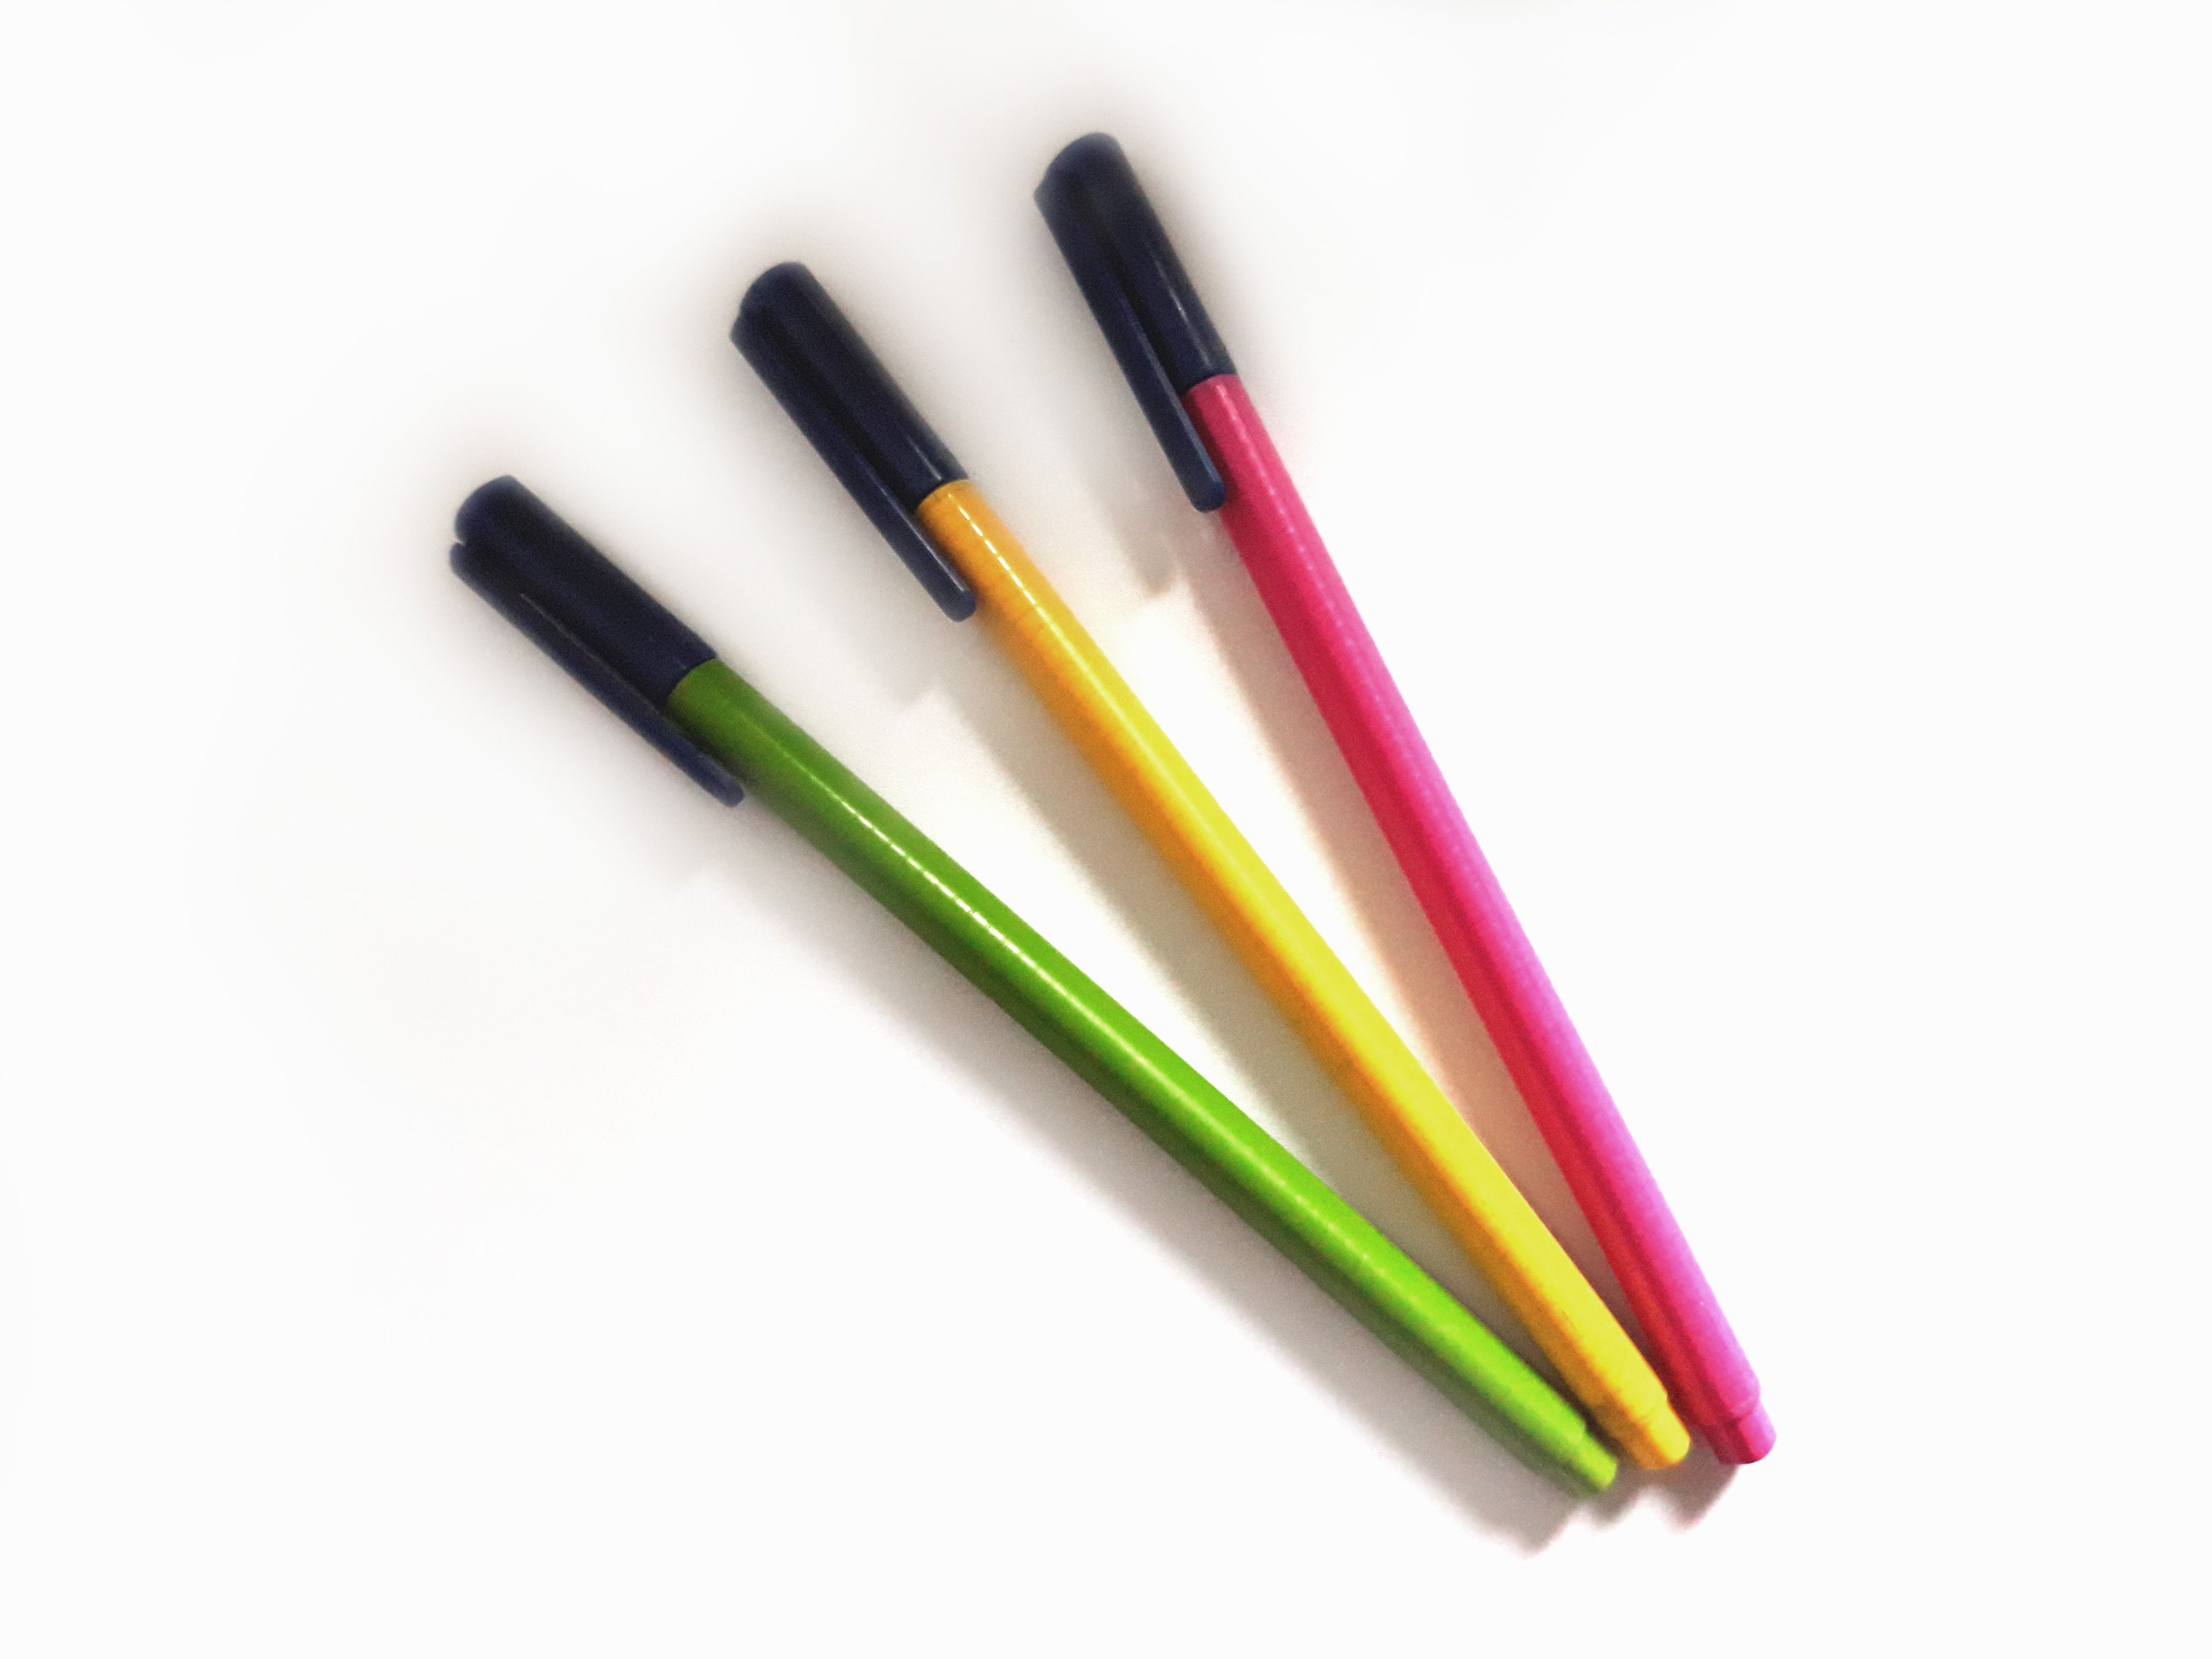
\includegraphics[width=5cm]{stift.jpg}
\caption*{Stifte}
}
\qquad
\begin{minipage}{5cm}
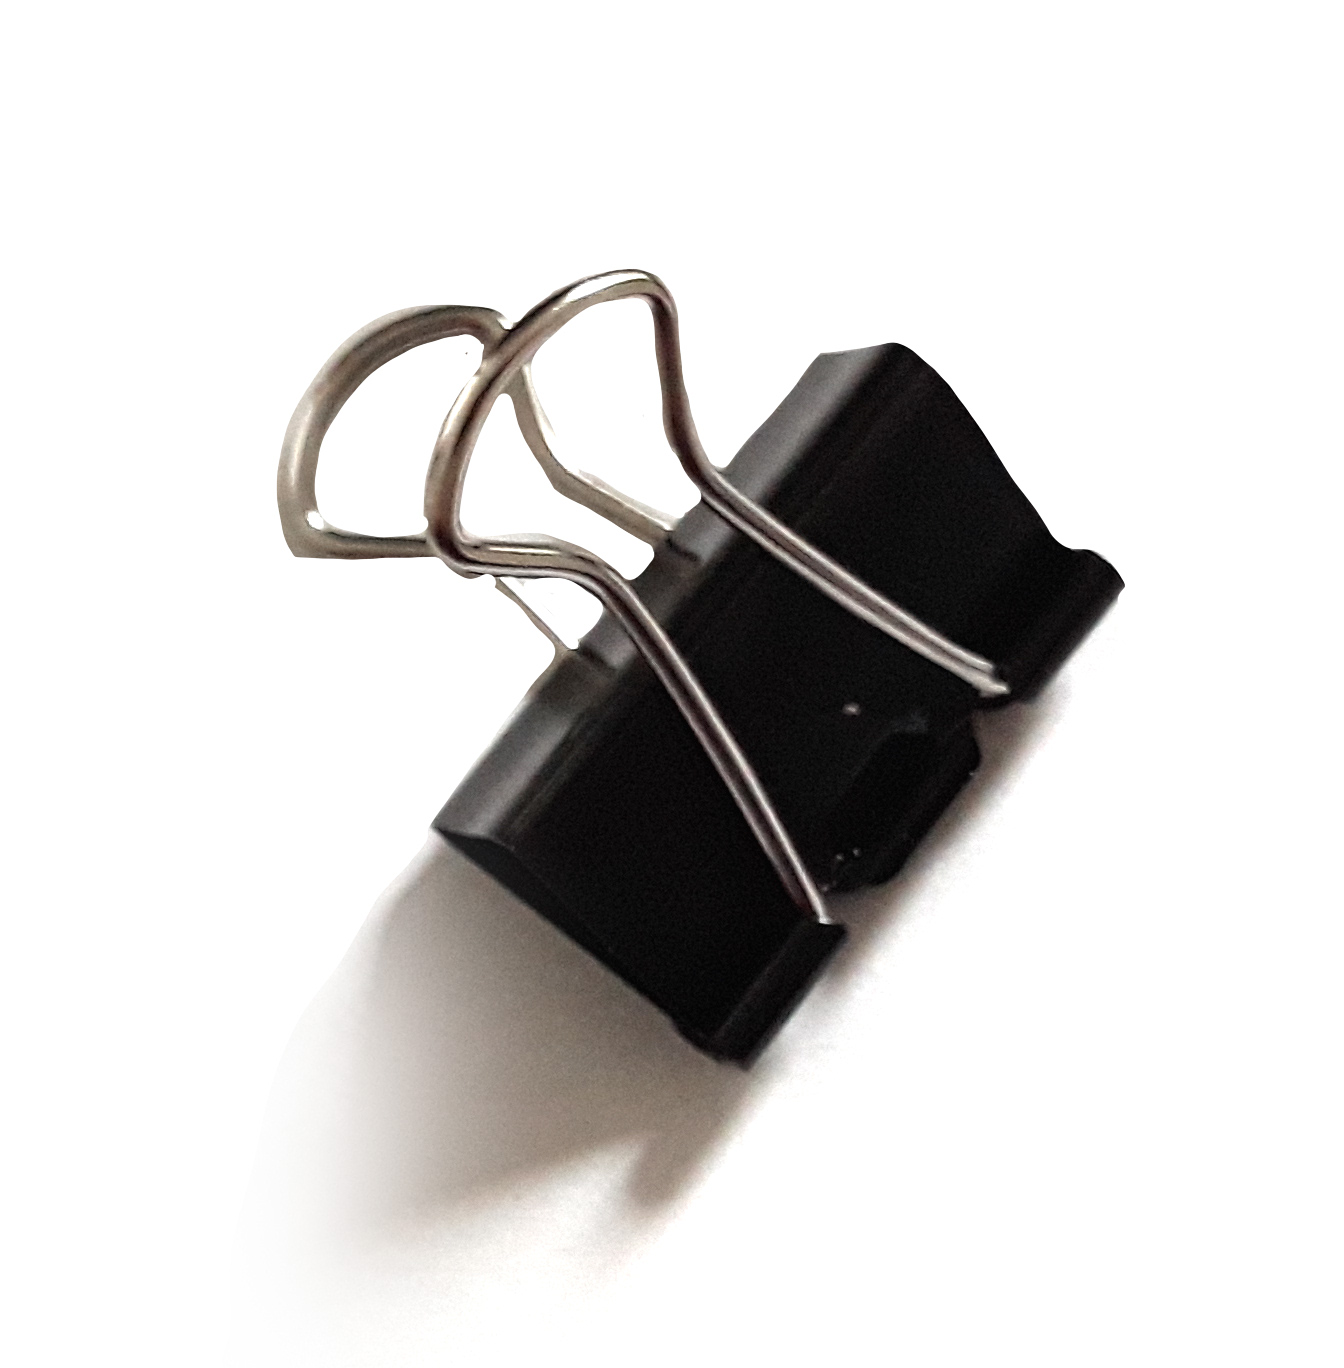
\includegraphics[width=5cm]{klammer.jpg}
\caption*{Klammer}
\end{minipage}
\end{figure}

\begin{figure}[h]
\centering
\parbox{5cm}{
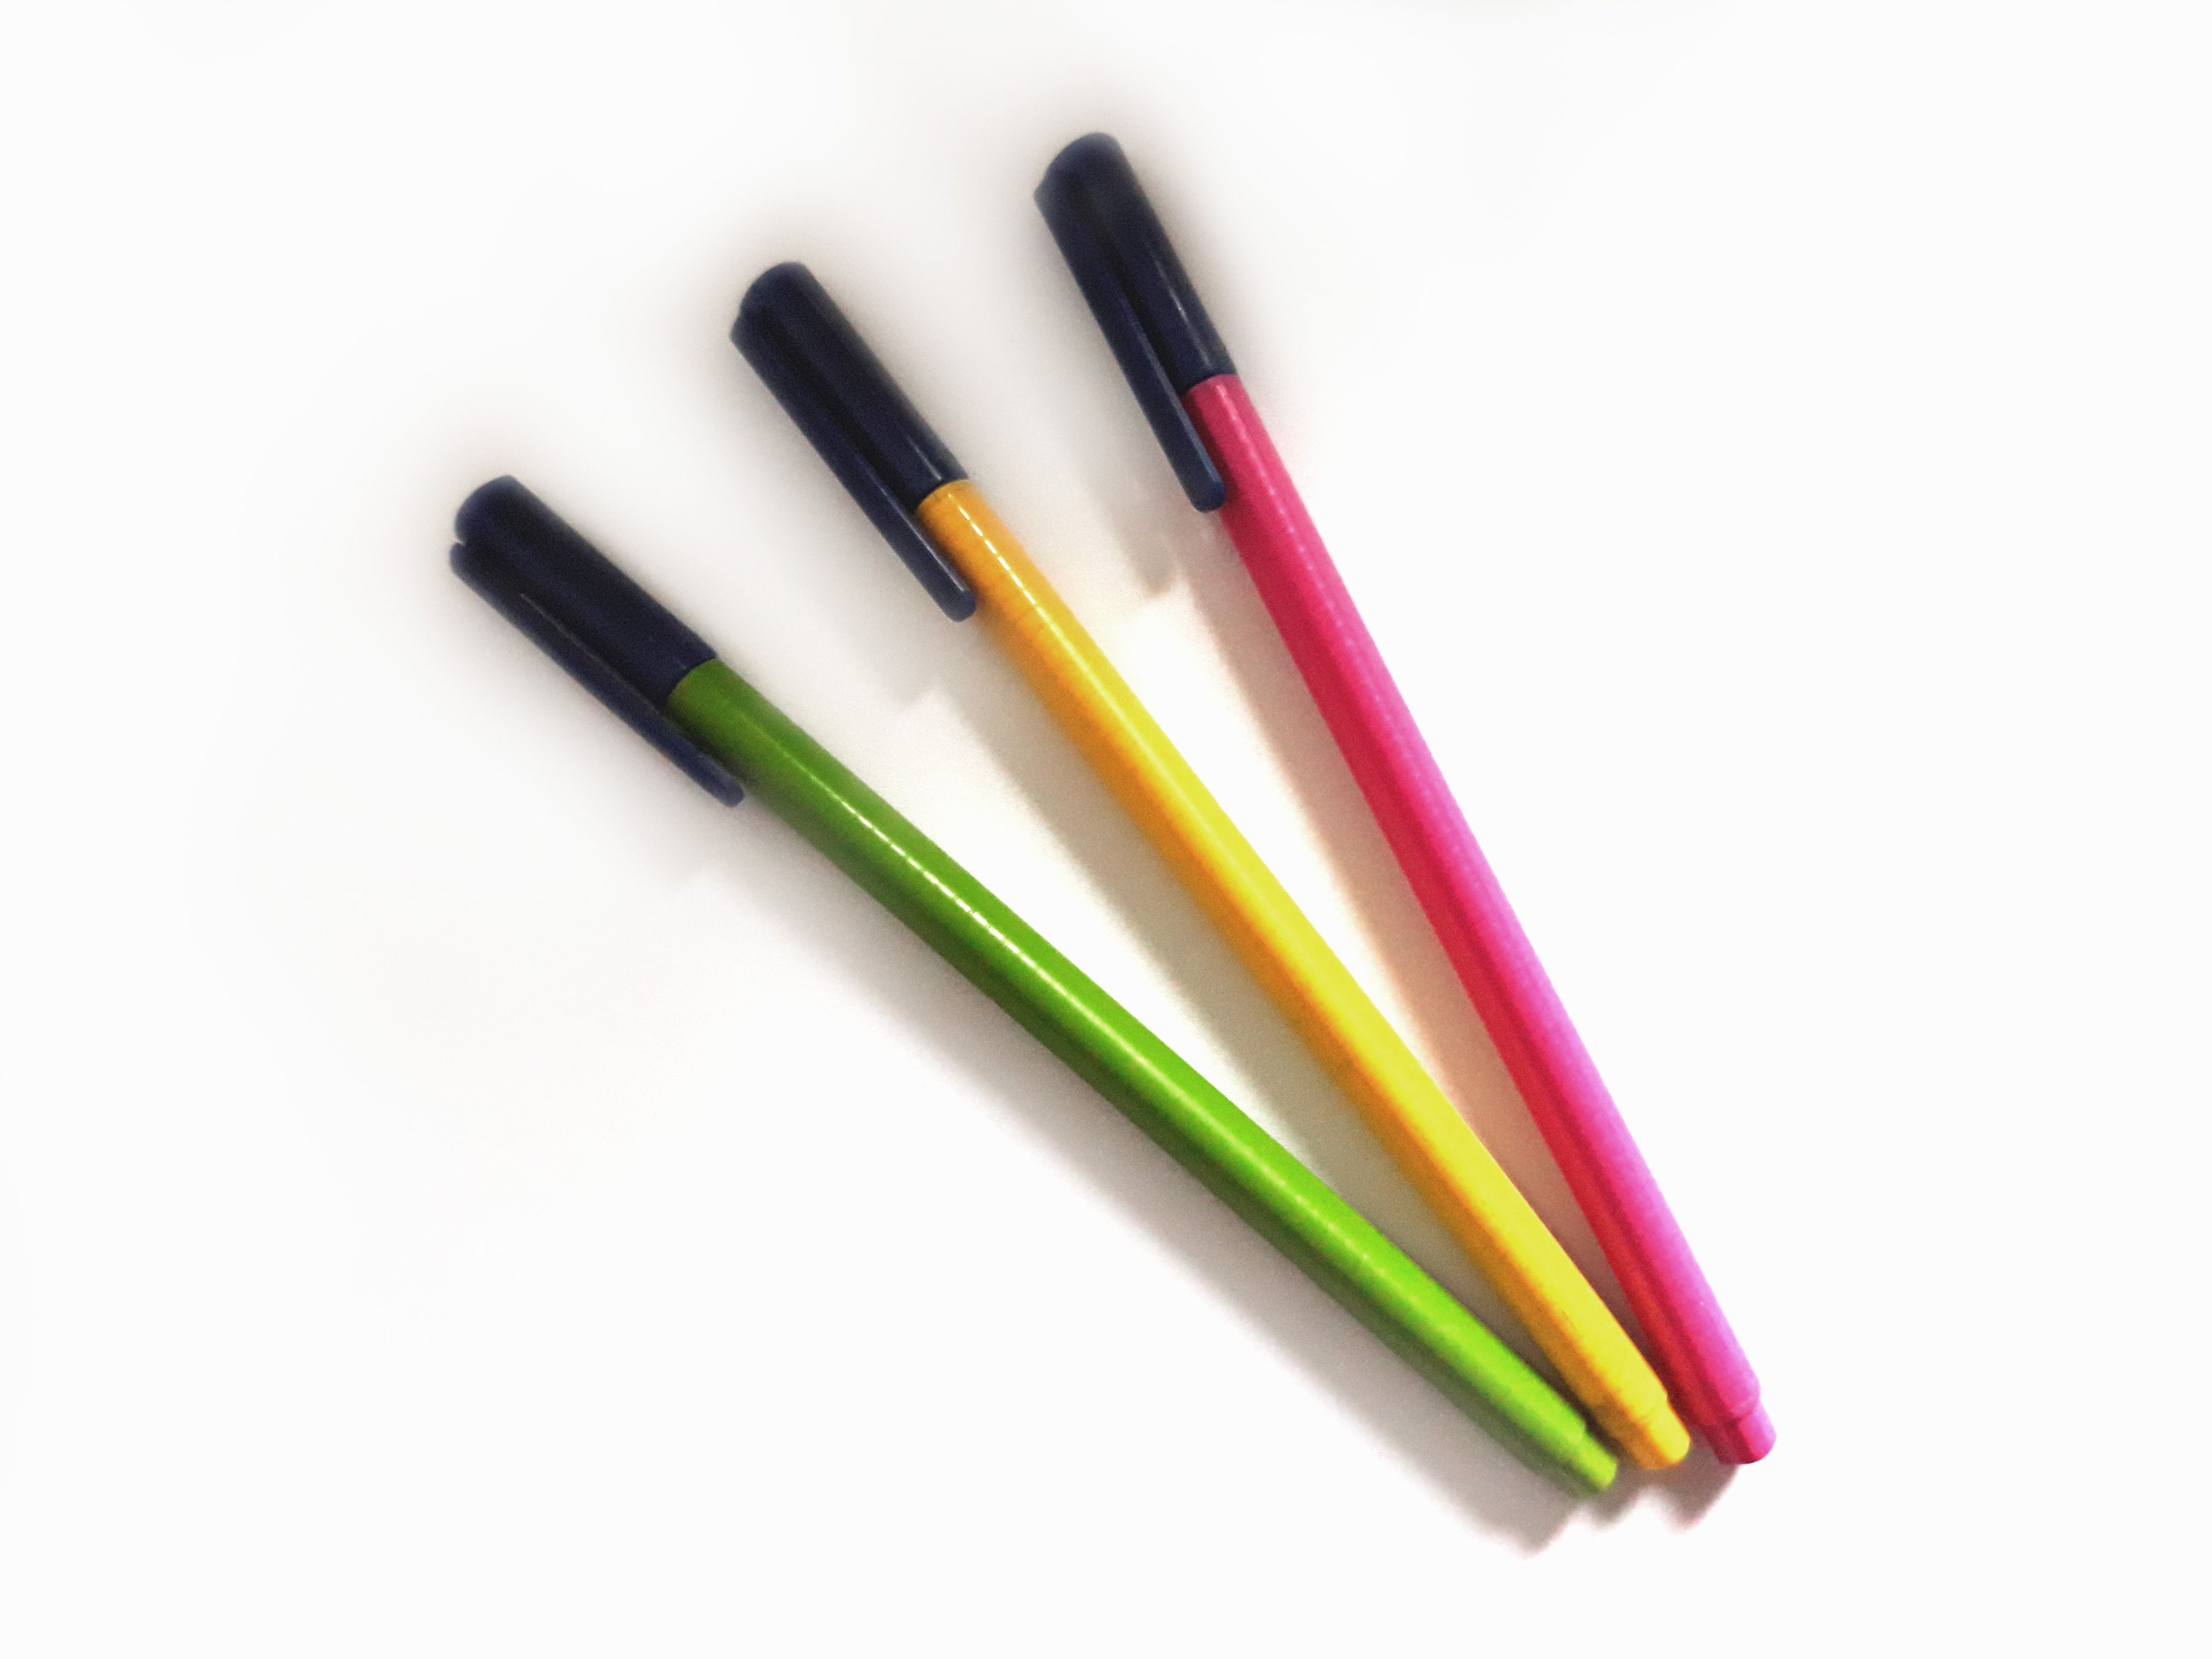
\includegraphics[width=5cm]{stift.jpg}
\caption*{Stifte}s
}
\hfill
\begin{minipage}{5cm}

\includegraphics[width=5cm]{mango.jpg}
\caption*{Mango 2}
\end{minipage}
\end{figure}

\subsection{Materialien}

\subsubsection{Werkzeuge}
\begin{checklist}
    \item Heißklebepistole
    \item Schere / Teppichmesser
    \item Schraubenzieher

    \begin{checklist}
    \item[] Optional:
    \item Abisolierzange
    \item Lötkolben
    \end{checklist}
\end{checklist}

\subsubsection{Material}
\begin{checklist}
    \item RaspberryPi
    \item Bildschirm + HDMI-Kabel
    \item Maus + Tastatur
    \item Zahnstocher
    \item Motoren
    \item L298N Motortreiber
    \item Pappe
    \item Kabel
    \item Räder
    \item Klammern
    \item Unterlage (Telefonbuch / Karton)
    \item X Female-Female Jumperkabel
    \item 1x Female-Male Jumperkabel
    \item 12 V Netzteil und Adapter
\end{checklist}


\subsection{Software}
Auf dem RaspberryPi sollte bereits ein funktionierendes \emph{Betriebssystem} installiert sein. Es bietet sich \emph{Raspberry Pi OS} (Raspbian) an. \\

Bei dem ursprünglichen Projekt wurde die Programmierumgebung \emph{Scratch} verwendet. Da diese die Ansteuerung von Motoren mit dem Raspberry Pi jedoch unnötig kompliziert macht, wurde hier auf die Verwendung der Programmiersprache \emph{Python} ausgewichen. Python bietet zwar keine grafische Programmieroberfläche (wie Scratch), ist jedoch, nach Meinung der Autoren, eine für alle Altersgruppen intuitive und mindestens genauso zugängliche Programmiermethode wie Scratch.\\

Zur Ausführung der Python-Skripte eignet sich eine Entwicklungsumgebung, wie z.B. \emph{Thonny} (vorinstalliert auf dem Pi).\\

Vorkenntnisse über Python sind nicht zwingend notwendig!

\subsubsection{Script}
Zur Vorbereitung sollten einige Funktionalitäten innerhalb von Python eingebaut werden, welche die Verwendung bei der Kursdurchführung für die Kursteilnehmer erleichtern. Die Nachfolgenden Programme sollten vorbereitet werden.\\

Auf dem Raspberry Pi im Filmbüro sollten diese Dateien bereits vorhanden sein. Sind sie es nicht, führen Sie die notwendigen Schritte im Anhang am Ende der Dokumentation aus.

